%%%%%%%%%%%%%%%%%%%%%%%%%%%%%%%%%%%%%%%%%
% Jacobs Landscape Poster
% LaTeX Template
% Version 1.0 (29/03/13)
%
% Created by:
% Computational Physics and Biophysics Group, Jacobs University
% https://teamwork.jacobs-university.de:8443/confluence/display/CoPandBiG/LaTeX+Poster
% 
% Further modified by:
% Nathaniel Johnston (nathaniel@njohnston.ca)
%
% This template has been downloaded from:
% http://www.LaTeXTemplates.com
%
% License:
% CC BY-NC-SA 3.0 (http://creativecommons.org/licenses/by-nc-sa/3.0/)
%
%%%%%%%%%%%%%%%%%%%%%%%%%%%%%%%%%%%%%%%%%


% Taken from above
% Liam Simmons - Apr 2018
% CSC 466 Poster Presentation

%----------------------------------------------------------------------------------------
%	PACKAGES AND OTHER DOCUMENT CONFIGURATIONS
%----------------------------------------------------------------------------------------

\documentclass[final]{beamer}

\usepackage[scale=1.24]{beamerposter} % Use the beamerposter package for laying out the poster
\usepackage{verbatim} % For comments
\usepackage{graphicx}


\usetheme{confposter} % Use the confposter theme supplied with this template

\setbeamercolor{block title}{fg=ngreen,bg=white} % Colors of the block titles
\setbeamercolor{block body}{fg=black,bg=white} % Colors of the body of blocks
\setbeamercolor{block alerted title}{fg=white,bg=dblue!70} % Colors of the highlighted block titles
\setbeamercolor{block alerted body}{fg=black,bg=dblue!10} % Colors of the body of highlighted blocks
% Many more colors are available for use in beamerthemeconfposter.sty

%-----------------------------------------------------------
% Define the column widths and overall poster size
% To set effective sepwid, onecolwid and twocolwid values, first choose how many columns you want and how much separation you want between columns
% In this template, the separation width chosen is 0.024 of the paper width and a 4-column layout
% onecolwid should therefore be (1-(# of columns+1)*sepwid)/# of columns e.g. (1-(4+1)*0.024)/4 = 0.22
% Set twocolwid to be (2*onecolwid)+sepwid = 0.464
% Set threecolwid to be (3*onecolwid)+2*sepwid = 0.708

\newlength{\sepwid}
\newlength{\onecolwid}
\newlength{\twocolwid}
\newlength{\threecolwid}
\setlength{\paperwidth}{48in} % A0 width: 46.8in
\setlength{\paperheight}{36in} % A0 height: 33.1in
\setlength{\sepwid}{0.024\paperwidth} % Separation width (white space) between columns
\setlength{\topmargin}{-0.5in} % Reduce the top margin size

%% 
% Lengths for 4-column layout

\setlength{\onecolwid}{0.22\paperwidth} % Width of one column
\setlength{\twocolwid}{0.464\paperwidth} % Width of two columns
\setlength{\threecolwid}{0.708\paperwidth} % Width of three columns
%%
% Lengths for 3-column layout
%\setlength{\onecolwid}{0.301\paperwidth} % Width of one column
%\setlength{\twocolwid}{0.627\paperwidth} % Width of two columns
%\setlength{\threecolwid}{0.952\paperwidth} % Width of three columns

%-----------------------------------------------------------

\usepackage{graphicx}  % Required for including images

\usepackage{booktabs} % Top and bottom rules for tables

%----------------------------------------------------------------------------------------
%	TITLE SECTION 
%----------------------------------------------------------------------------------------

\title{A Replicable and Extensible Comparison of QUIC and TCP} % Poster title

\author{Henry Baxter and Liam Simmons} % Author(s)

\institute{University of Victoria - CSC 466} % Institution(s)

%----------------------------------------------------------------------------------------

\begin{document}

\addtobeamertemplate{block end}{}{\vspace*{2ex}} % White space under blocks
\addtobeamertemplate{block alerted end}{}{\vspace*{2ex}} % White space under highlighted (alert) blocks

\setlength{\belowcaptionskip}{2ex} % White space under figures
\setlength\belowdisplayshortskip{2ex} % White space under equations

\begin{frame}[t] % The whole poster is enclosed in one beamer frame

\begin{columns}[t] % The whole poster consists of three major columns, the second of which is split into two columns twice - the [t] option aligns each column's content to the top

\begin{column}{\sepwid}\end{column} % Empty spacer column

\begin{column}{\onecolwid} % The first column

%----------------------------------------------------------------------------------------
%	What is QUIC? What are the feature of QUIC?
%----------------------------------------------------------------------------------------

\begin{block}{What is QUIC?}

QUIC is an encrypted, multiplexed, low latency protocol that was designed to improve HTTPS traffic. \cite{Langley:2017:QTP:3098822.3098842} As of 2017, QUIC accounts for 7\% of all internet traffic. \cite{Kakhki:2017:TLL:3131365.3131368}

\end{block}

\begin{block}{What are the features of QUIC?}

\begin{figure}
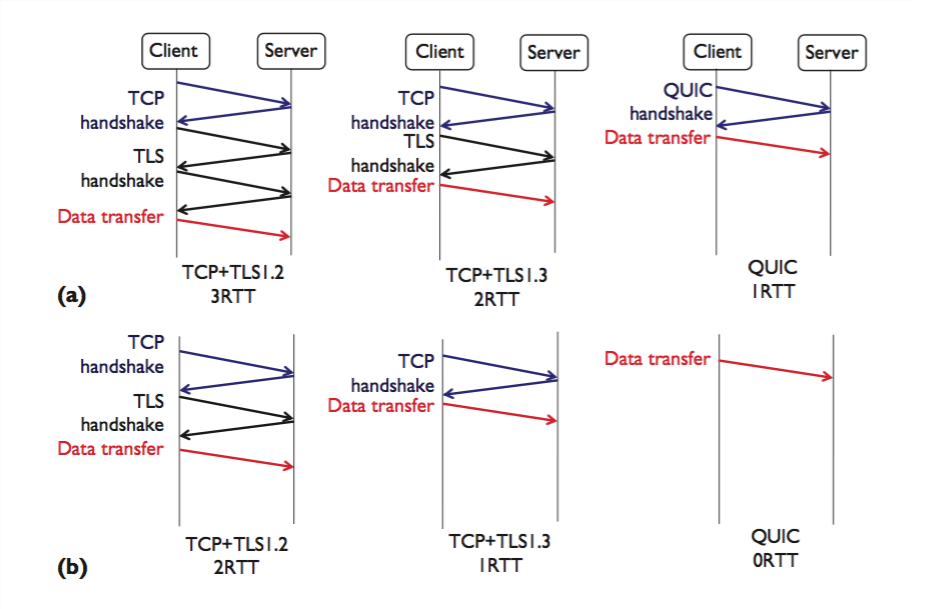
\includegraphics[width=0.8\linewidth]{images/QUIC_TCP_RTT.png}
\caption{Handshake RTT of different protocols. (a) First-time connection establishment (b) Subsequent connections. Image credit \cite{7867726}}
\end{figure}

\begin{itemize}
	\item \textbf{0-RTT:} QUIC features 0-RTT connection re-establishment by using cached cryptographic session information.
	\item \textbf{Stream Multiplexing:} QUIC allows multiple streams across one flow, which avoids head-of-line blocking found in TCP
	\item \textbf{Congestion Control, Loss Recovery:} QUIC uses unique sequence numbers, to help distinguish retransmissions from original packets
\end{itemize}


\begin{figure}
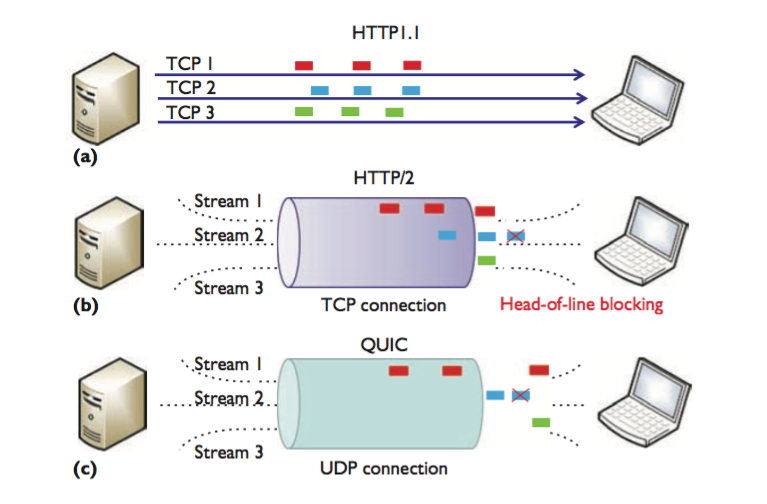
\includegraphics[width=0.8\linewidth]{images/QUICmulti.png}
\caption{Multiplexing comparison over (a) HTTP1.1 (b) HTTP/2 and (c) QUIC. Image credit \cite{7867726}}
\end{figure}

\end{block}
%----------------------------------------------------------------------------------------

\end{column} % End of the first column

\begin{column}{\sepwid}\end{column} % Empty spacer column

\begin{column}{\onecolwid} % The first column within column 2 (column 2.1)

%----------------------------------------------------------------------------------------
%	Experimental Design
%----------------------------------------------------------------------------------------
\begin{block}{Motivation}
\begin{itemize}
	\item QUIC is a rapidly evolving protocol
	\item Analysis of QUIC is limitied, as compared to TCP
	\item Focusing on replicability and extensibility, this study will allow for tracking protocol changes as they are made
\end{itemize}
\end{block}

\begin{block}{Experimental Design}

\textbf{Flow of test session}

\begin{itemize}
	\item Parallel instances of Chrome are launched on a local machine or a \textit{desktop} EC2 instance
	\item Treatments are generated from a configuration file, including variations in pages requested and network conditions
	\item When a treatment is run the test environment is automatically configured
	\item Requests are initiated programatically and page load time is captured for multiple runs
	\item Treatment data is saved, aggreated, plotted and analyzed
\end{itemize}

\begin{figure}
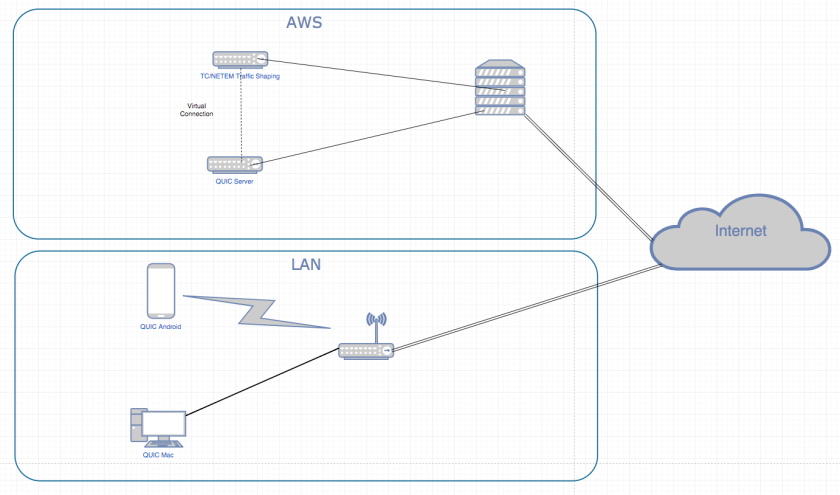
\includegraphics[width=0.8\linewidth]{images/Network_diagram.png}
\caption{Testbed Setup}
\end{figure}

\textbf{Organization of testbed}

\begin{itemize}
	\item Requests are routed through a \textit{router} EC2 instance
	\item TCP and QUIC requests are handled by a \textit{server} EC2 instance
	\item All EC2 instances are on the same private LAN
	\item The router forwards with iptables and shapes traffic with tc htb and qdisc
	\item The entire process is configurable and automatic	
\end{itemize}

\end{block}

\end{column} % End of column 2.1

%----------------------------------------------------------------------------------------

\begin{column}{\onecolwid}% The second column within column 2 (column 2.2)

%\begin{block}{Data and Results}\end{block}

\begin{block}{Object Number and Size}
\begin{figure}
\begin{tabular}{c c}
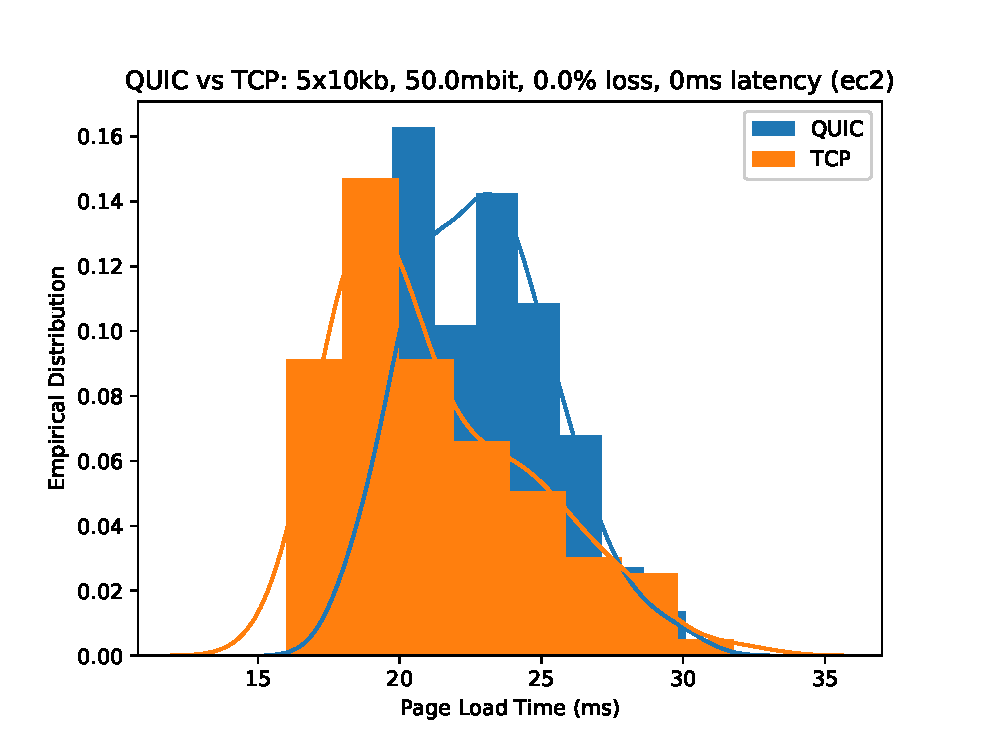
\includegraphics[width=0.4\linewidth]{{plots/local/5n-10k-50.0mbit-0.0loss-0ms}.eps} &
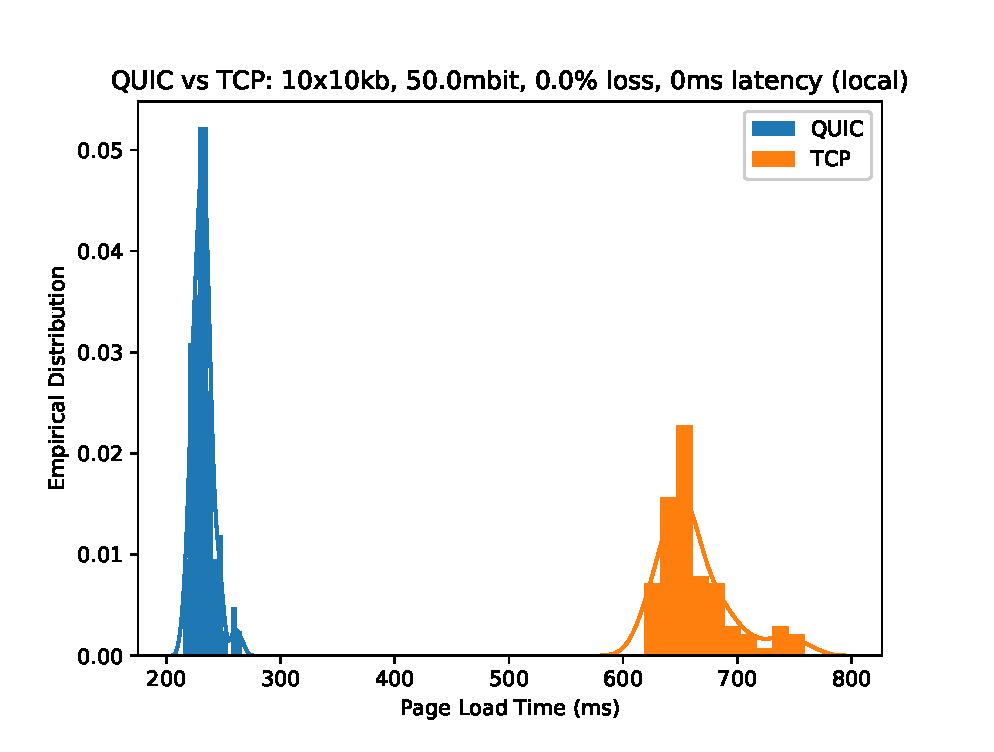
\includegraphics[width=0.4\linewidth]{{plots/local/10n-10k-50.0mbit-0.0loss-0ms}.eps} \\
\tiny (a) & \tiny (b) \\
\end{tabular}
\caption{QUIC vs TCP for (a) 5 (b) 10 objects}
\end{figure}

\begin{figure}
\begin{tabular}{c c}
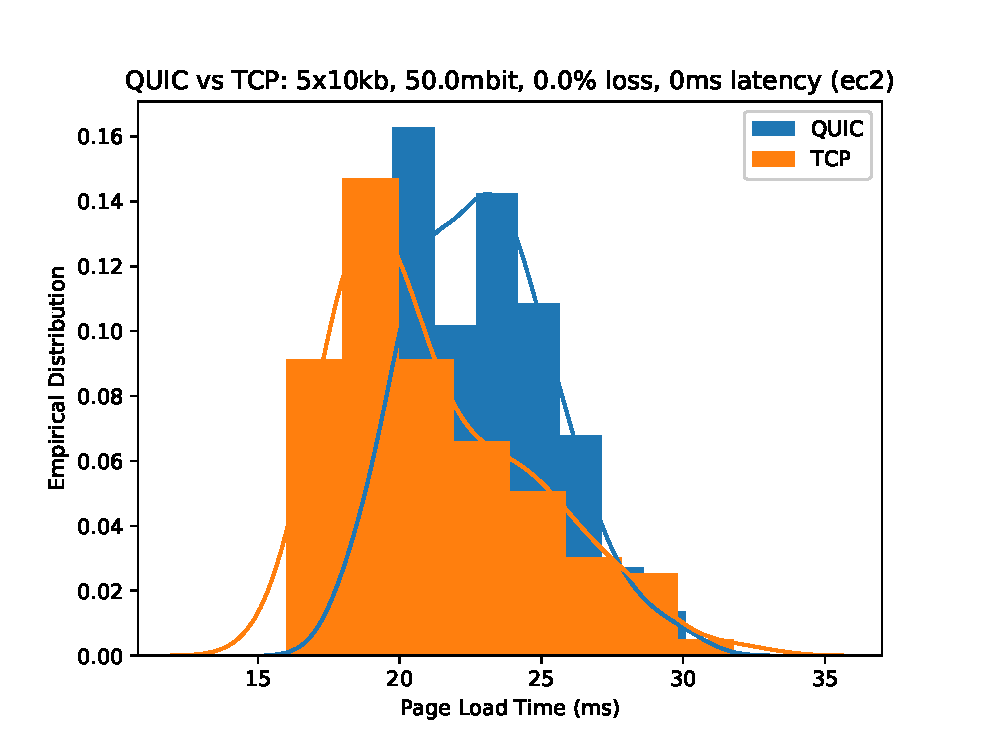
\includegraphics[width=0.4\linewidth]{{plots/local/5n-10k-50.0mbit-0.0loss-0ms}.eps} &
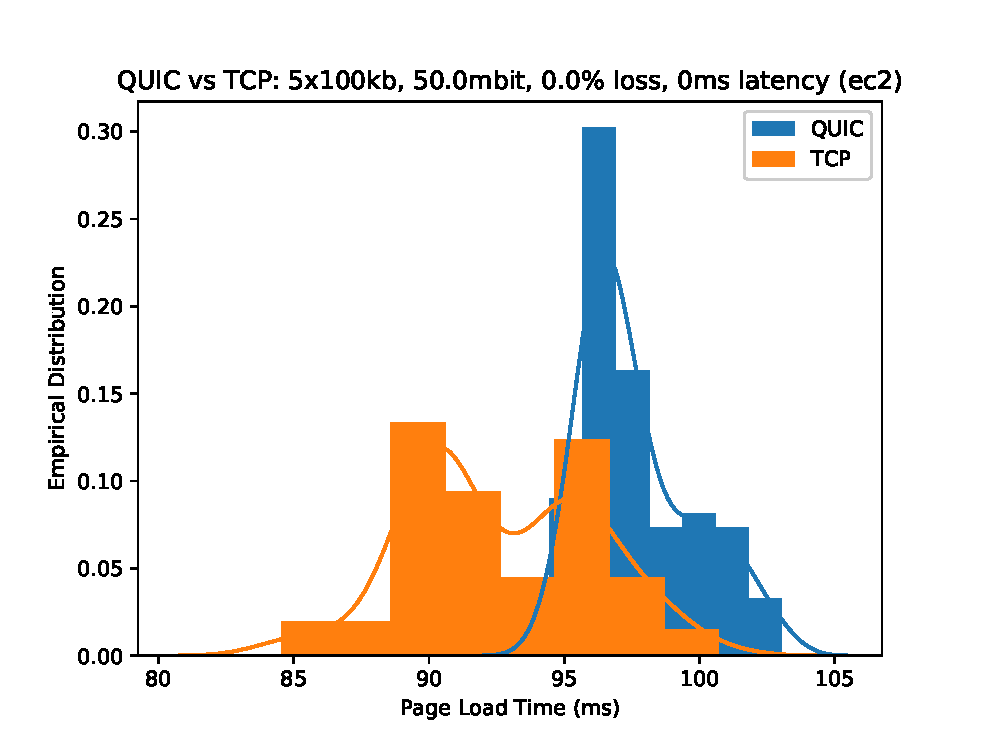
\includegraphics[width=0.4\linewidth]{{plots/local/5n-100k-50.0mbit-0.0loss-0ms}.eps} \\
\tiny (a) & \tiny (b) \\
\end{tabular}
\caption{QUIC vs TCP for (a) 10kB (b) 100kB objects}
\end{figure}
\end{block}

\begin{block}{Internet vs EC2 VLAN}
\begin{figure}
\begin{tabular}{c c}
\includegraphics[width=0.4\linewidth]{{plots/local/packet-loss}.eps} &
\includegraphics[width=0.4\linewidth]{{plots/ec2/packet-loss}.eps} \\
\tiny (a) & \tiny(b) \\
\includegraphics[width=0.4\linewidth]{{plots/local/latency}.eps} &
\includegraphics[width=0.4\linewidth]{{plots/ec2/latency}.eps} \\
\tiny (c) & \tiny(d) \\
\includegraphics[width=0.4\linewidth]{{plots/local/object-count}.eps} &
\includegraphics[width=0.4\linewidth]{{plots/ec2/object-count}.eps} \\
\tiny (e) & \tiny(f) \\
\end{tabular}
\caption{Varying packet loss, latency, and object count for local (a), (c) and (e) respectively, and EC2 instance (b), (d) and (f)}
\end{figure}
\end{block}

\end{column} % End of column 2.2

\begin{column}{\sepwid}\end{column} % Empty spacer column

\begin{column}{\onecolwid} % The third column

%----------------------------------------------------------------------------------------
%	CONCLUSION
%----------------------------------------------------------------------------------------



\begin{block}{Conclusion}

\textbf{Current results}

\begin{itemize}
\item For all variables tested, QUIC outperforms TCP \textit{from the local client}
\item With one exception, for very large numbers of objects, TCP is faster
\item When requesting from an EC2 instance on the same VLAN, TCP is faster
\item This suggests that QUIC performs best for a consumer in most situations
\item It may suggest some optimization of TCP/IP performance in VLANs for AWS, perhaps in regard to shared VMs on a physical host
\end{itemize}

\textbf{Next steps}
\begin{itemize}
	\item Further tests with iperf in the AWS cloud
	\item Side traffic tests to compare fairness
	\item Jitter impact
	\item Packet reordering
\end{itemize}

Given the extensible and reproducible framework created, it is possible to add most of these tests with very minimal work.

\end{block}

%----------------------------------------------------------------------------------------
%	REFERENCES
%----------------------------------------------------------------------------------------

\begin{block}{References}

\nocite{*} % Insert publications even if they are not cited in the poster
\small{\bibliographystyle{unsrt}
\bibliography{bibliography}\vspace{0.75in}}

\end{block}

%----------------------------------------------------------------------------------------

\end{column} % End of the third column
\end{columns} % End of all the columns in the poster
\end{frame} % End of the enclosing frame

\end{document}
